% Chapter 5

\chapter{Conclusions and Future Work} % Main chapter title

\label{Chapter6} % For referencing the chapter elsewhere, use \ref{Chapter5} 

%----------------------------------------------------------------------------------------


%----------------------------------------------------------------------------------------

\section{Conclusions}
The present work provides a well-known iterative scheme -- classical Benders' decomposition -- to solve large combinatorial optimization problems. Specifically, we provided an implementation of BD that combines quantum and classical solvers. We formulated a general TEP problem by taking into account investment cost, load shedding cost and operational cost and split the original problem into a master problem in QUBO formulation, tackled by the quantum solver, and a slave problem, tackled by the classical solver. The quantum solver is a quantum annealer and the classical solver is any of the well-known classical methods such as simplex or the interior point method to solve the slave problem. Benders' decomposition has convergence properties so that we could control how good a solution to a combinatorial problem is by comparing the difference between an upper and a lower bound. Furthermore, we could control the degree to which the quantum solver is employed in the algorithm, opening up the possibility of increasing the complexity of the problem assigned to the quantum solver according to the hardware evolution. Currently, hybrid approaches, such as the ones from D-Wave, provide the solution to large combinatorial optimization problem where there are binary, integer and even real variables involved. However, we cannot know how much quantum solver we used in the resolution of our problem. The problems solved in this thesis with those hybrid solvers are intended to be the test cases for the implementation of the quantum BD algorithm, which is left for future work. It is our belief that a specific hybrid implementation would solve the problem faster and better than a general hybrid approach as that of D-Wave.\\\\
The potential speed-up would help to close the granularity gap between what the current models can solve and the desired solutions needed by energy system operators. Tackling real-time problems by using the smart grid data is still far from being solved efficiently by classical and quantum solvers but iterative methods open a new path to explore the resolution of large problems in shorter times by gaining speed-up from the quantum solvers.\\\\
This work aims to show the challenges of applying hybrid quantum-classical methods to energy sector problems. It is our belief that, although quantum solvers are still in their early stages, hybrid approaches will allow researchers and different industry players to unlock the potential of current quantum solvers.
%%%%%
\section{Future Work}
This master thesis has presented an iterative approach to solve TEP problems. We plan to implement the quantum BD in Python and use real data from different sources of energy models to develop the test cases. Depending on the source from which we load the data we need to process it accordingly. We will use the PyPSA python package\,\cite{PyPSA-Eur:PyPSA-Eur} to take care of that issue.\\\\
Dealing with real data implies not only dealing with real numbers -- that can be rounded to integers -- but also with a large number of variables which increase the complexity of the problem. These points do not change the implementation, but if we plan to add new components such as storages -- which implies taking into account a multi-snapshot dependence -- the linear equations that describe our problem are going to change. PyPSA can simplify the linear model for any number of targets considered in the original problem and to plot the associated network for a given number of nodes $N$, as in Figure\,\ref{fig:GeneralNetworks}. This enables us to read these linear equations and include them into our Benders' decomposition scheme. For this task we plan to use QUARK\,\cite{dlrsc2023quark}, a reformulation kernel that allows us to send the algorithm to different quantum machines.
\begin{figure}[H]
\centering
\begin{subfigure}[c]{0.5\linewidth}
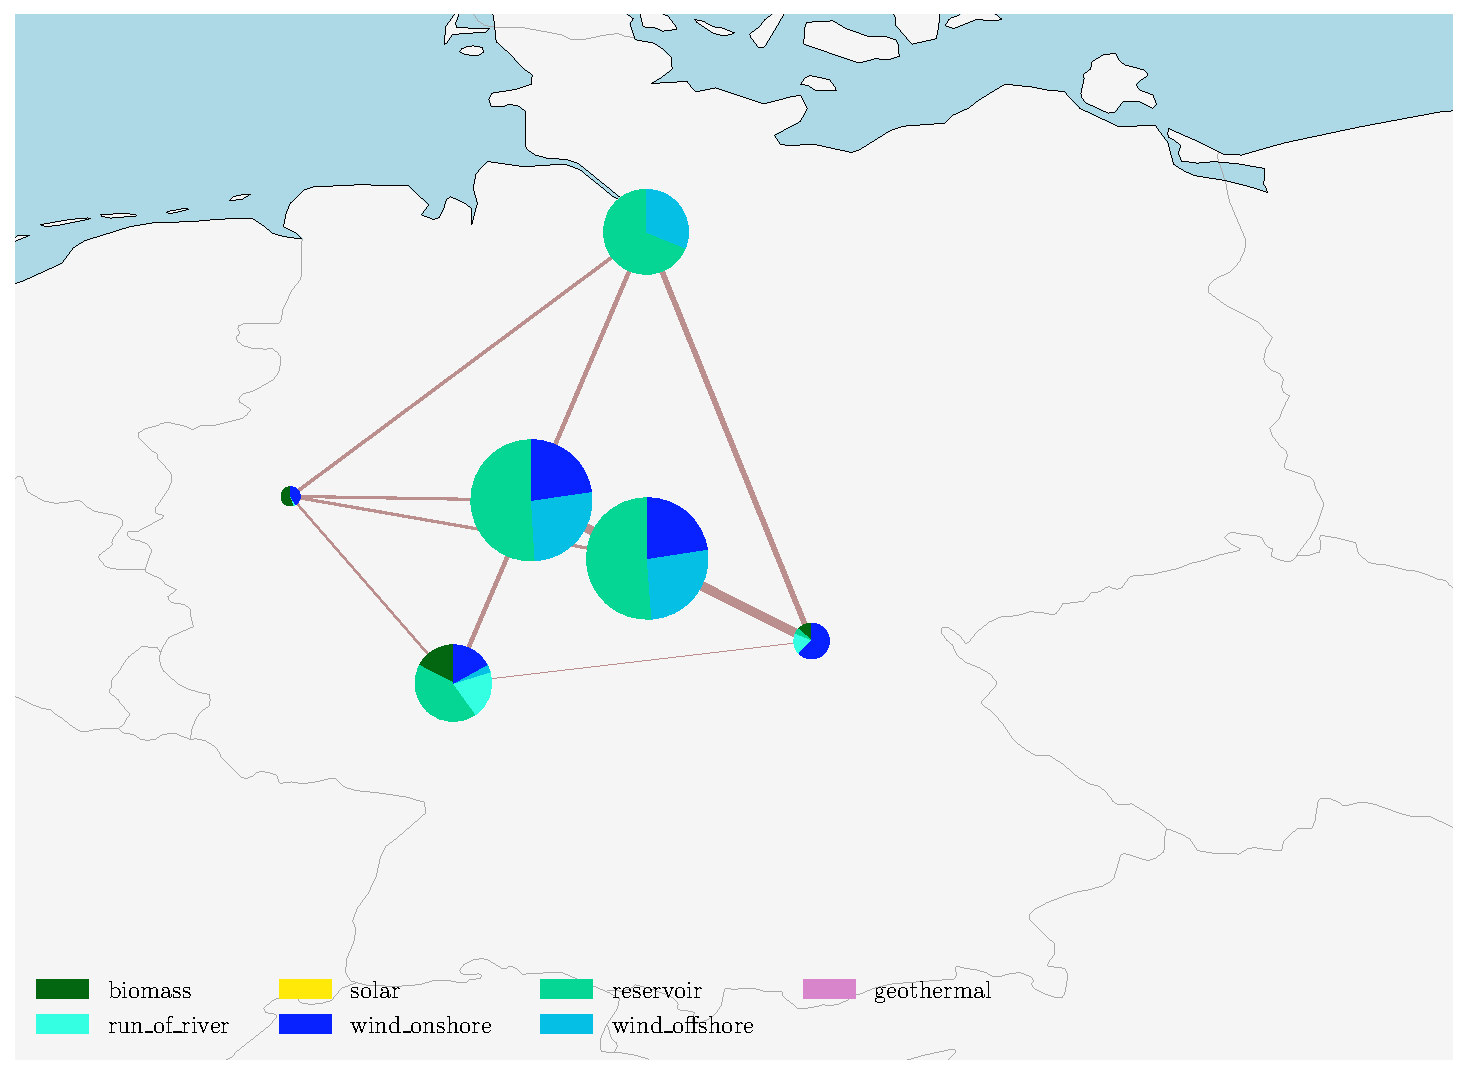
\includegraphics[width=\linewidth]{Figures/eGo100_No4.pdf} 
\caption{$N=6$.}
\label{fig:3a}
\end{subfigure}\hfill    
\begin{subfigure}[c]{0.5\linewidth}
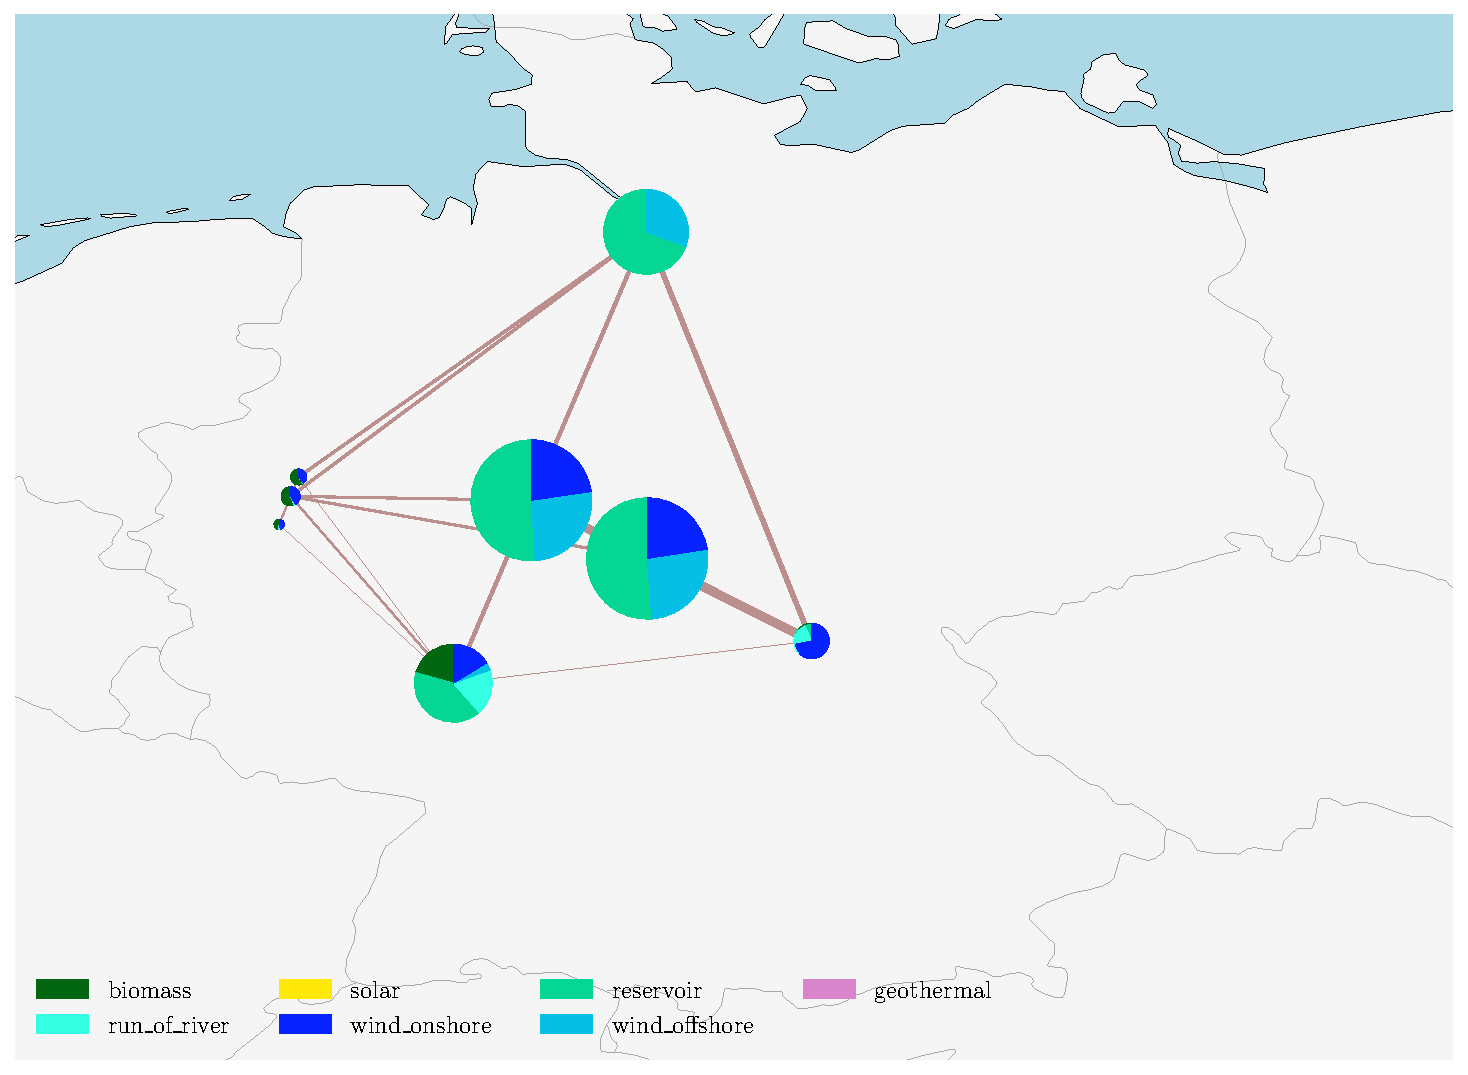
\includegraphics[width=\linewidth]{Figures/eGo100_No5.pdf}
\caption{$N=8$.}
\label{fig:3b}
\end{subfigure}
%add desired spacing between images, e. g. ~, \quad, \qquad, \hfill etc. 
%(or a blank line to force the subfigure onto a new line)
\begin{subfigure}[c]{0.5\linewidth}
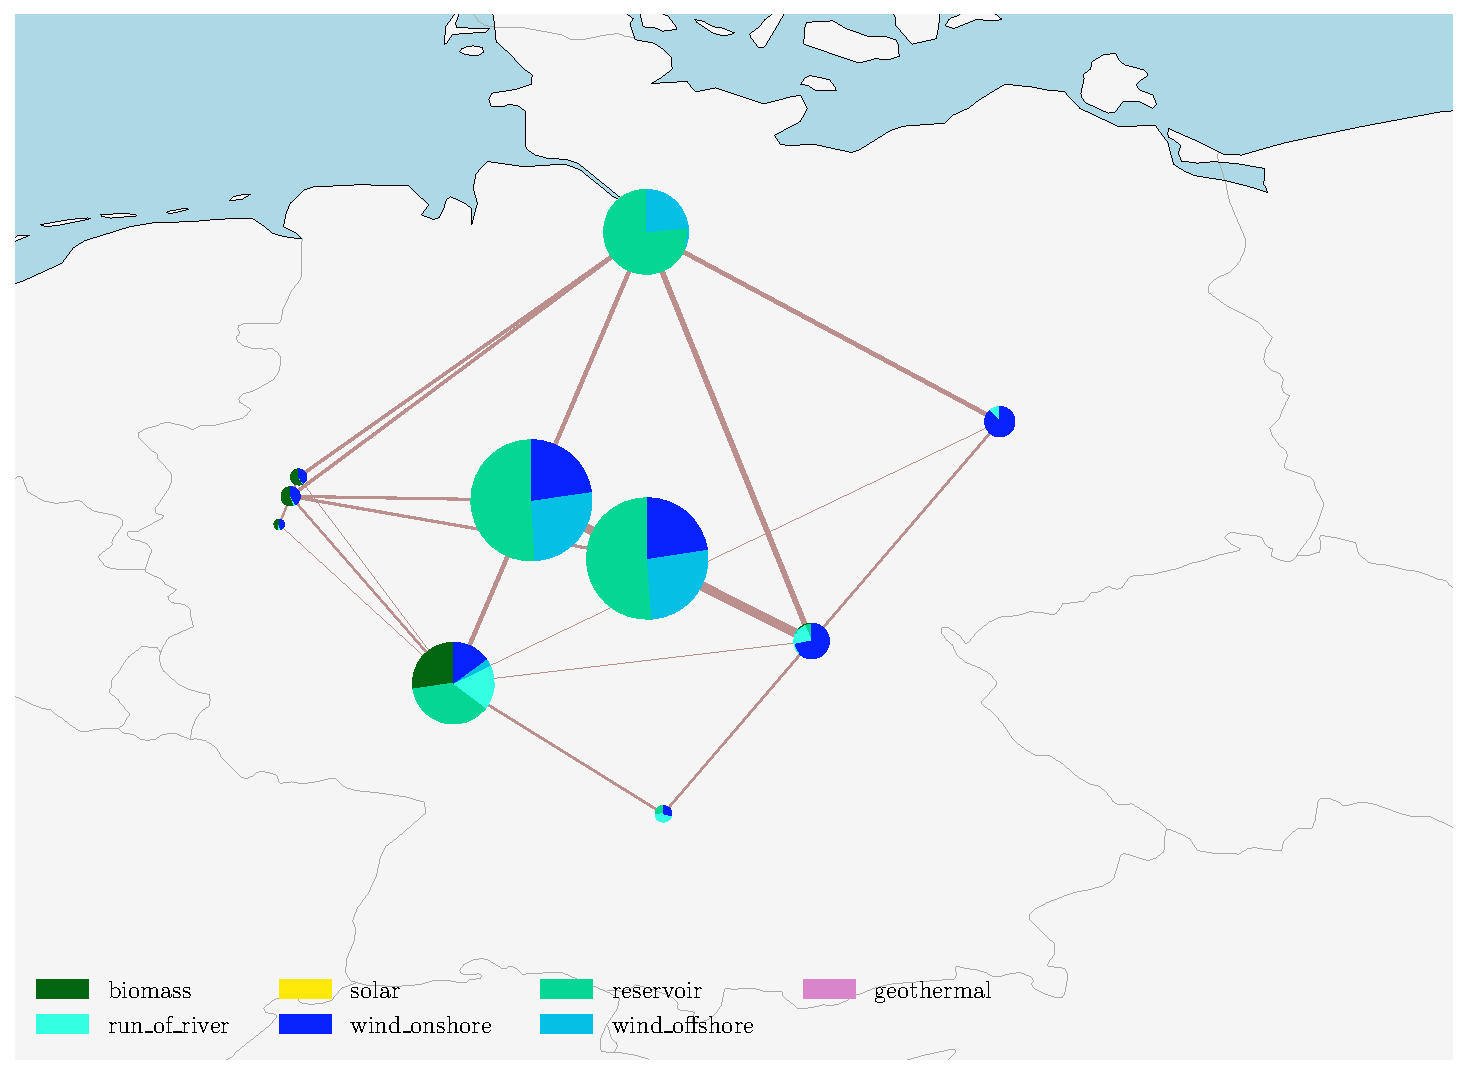
\includegraphics[width=\linewidth]{Figures/eGo100_No6.pdf}
\caption{$N=10$.}
\label{fig:3c}
\end{subfigure}\hfill    
\begin{subfigure}[c]{0.5\linewidth}
\includegraphics[width=\linewidth]{Figures/eGo100_No7.pdf}
\caption{$N=12$.}
\label{fig:3d}
\end{subfigure}
    
\caption{Germany network generated with PyPSA for $N$ clusters from eGo100 data\,\cite{Mueller2018}.}
\label{fig:GeneralNetworks}
\end{figure}
Last, we could compare our hybrid quantum-classical algorithm with the ones provided by the quantum solvers. We think that a specific hybrid quantum-classical approach should provide a better solution in terms of computational time and optimal value than the general hybrid solvers from D-Wave. Furthermore, we should be able to determine the exact usage of quantum solver we are employing in the problem, which is not possible with solvers such as D-Wave.